\documentclass[12pt]{article}

\usepackage{fullpage}
\usepackage[utf8]{inputenc}
\usepackage[T1]{fontenc}
\usepackage{indentfirst}
\usepackage{graphicx}
\usepackage{booktabs}
\graphicspath{ {images/} }
\usepackage[portuguese]{babel} % Mul­tilin­gual sup­port for Plain TEX or LaTeX.

\begin{document}
\begin{titlepage}
    
\includegraphics[width=0.3\textwidth]{fctUnlLogo.jpg}
    \begin{center}
        \vspace{0.5cm}

        \begin{Large}
        	\underline{\textbf{Opção A}}\\
        \end{Large}
        
        \textbf{\emph{Publish-Subscribe using Structured}}
               
        \vspace{0.3cm}

		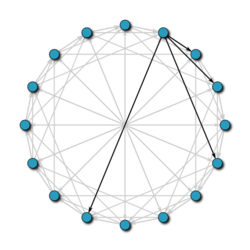
\includegraphics[width=0.4\textwidth]{Chord_network.png}
		
        \vspace{0.3cm}
        
        Trabalho realizado por:
        
        \vspace{0.5cm}

		\begin{table}[htbp]
		\centering
        	\begin{tabular}{c c}
				\textbf{Luís Duarte Oliveira, nº 41894} & \textbf{Daniel Pimenta, nº 45404}\\
				\texttt{ld.oliveira@campus.fct.unl.pt} & \texttt{d.pimenta@campus.fct.unl.pt}\\
			\end{tabular}
		\end{table}
		
		\begin{table}[htbp]
		\centering
        	\begin{tabular}{c}
				\textbf{Luís Martins, nº 45640}\\
				\texttt{lg.martins@campus.fct.unl.pt}\\
			\end{tabular}
		\end{table}
		
        \vspace{0.5cm}
        
        Para a cadeira de:
        
        Algoritmos e Sistemas Distribuídos (ASD)
        
        \vspace{0.5cm}

		Professor regente: 
		João Leitão
		
		Professor responsável:
		Nuno Preguiça
		
        \vspace{0.5cm}
                
        Departamento de Informática\\
        Faculdade de Ciências e Tecnologia\\
        Universidade Nova de Lisboa\\
        17 de novembro de 2018
    \end{center}
\end{titlepage}

\newpage
\tableofcontents

\newpage
\listoffigures

\newpage
\listoftables

\newpage
\section{Resumo}

TO DO...

\newpage
\section{Introdução}

Com o aparecimento e evolução da Internet existiu uma enorme evolução dos modelos de comunicação utilizados pelos sistemas de computadores. Estes modelos podem ser divididos em dois grandes grupos, os modelos de sistemas centralizados em que na sua variação mais simples, os clientes comunicam com um servidor que satisfaz todos os seus pedidos, e os modelos de sistemas distribuídos em que o sistema é feito de nós que representam vários pontos de uma rede onde existem nós que são clientes e outros que são servidores (por vezes os clientes podem também ser servidores). Os nós servidores podem ser replicas perfeitas uns dos outros ou apenas fazerem uma replicação parcial das operações fornecidas. Desta forma não existe um único ponto de falha e existe uma divisão do trabalho pelos vários nós do sistema. Os sistemas distribuídos são bastante complexos e têm várias propriedades. A realização deste trabalho tem como base a implementação de um sistema distribuído estruturado, ou seja, os nós da rede estão organizados segundo uma determinada ordem, sendo a ordem mais comum representada por uma forma em anel.

\newpage
\section{Objetivos}

O objetivo deste estudo é a implementação de um sistema de subscrição montado em cima de um sistema distribuído estruturado conhecido por tabela de dispersão distribuída (DHT). Com a programação deste sistema, temos a oportunidade de estudar os pormenores da sua implementação e de aprender a realizar testes de desempenho e de fiabilidade a um sistema destes.

\newpage
\section{Implementação}

A implementação desta DHT tem como base o algoritmo de Chord tal como visto no artigo \cite{b2} e o sistema de subscrição tem como base o os materiais da cadeira \cite{b1}. A programação deste sistema foi feita com a linguagem computacional de Scala \cite{b3} e utilizando o conjunto de ferramentas do Akka \cite{b4}.

\newpage
\section{Testes}

Os testes ao sistema têm como objetivo a analise do desempenho e da fiabilidade do mesmo. Para isso serão recolhidos dados lançando 100, 1000 e 10000 nós.

\subsection{Teste dos 100 nós}

TO DO...

\subsection{Teste dos 1000 nós}

TO DO...

\subsection{Teste dos 10000 nós}

TO DO...

\newpage
\section{Conclusões}

TO DO...

\newpage
\begin{thebibliography}{00}
\bibitem{b1} Leitão, J. (2018). Materiais da cadeira de ASD. FCT/UNL.
\bibitem{b2} Stoica, I., Morris, R., Liben-Nowell, D., Karger, D. R., Kaashoek, M. F., Dabek, F., \& Balakrishnan, H. (2003). Chord: A scalable peer-to-peer lookup protocol for Internet applications. IEEE/ACM Transactions on Networking, 11(1), 17–32. https://doi.org/10.1109/TNET.2002.808407
\bibitem{b3} Fédérale, É. P., \& (EPFL), L. (n.d.). Scala. Retrieved November 17, 2018, from https://www.scala-lang.org/
\bibitem{b4} Lightbend, I. (n.d.). Akka. Retrieved November 17, 2018, from https://akka.io/
\bibitem{b5} Penman, T. (n.d.). Implementing a Distributed Hash Table with Scala and Akka. Retrieved November 17, 2018, from http://tristanpenman.com/blog/posts/2015/11/26/implementing-a-dht-with-scala-and-akka/
\end{thebibliography}

\end{document}